\documentclass[a4paper,12pt]{scrartcl}
\usepackage[utf8]{inputenc}
\usepackage[ngerman]{babel}
\usepackage[T1]{fontenc}
\usepackage{amsmath}
\usepackage{stmaryrd}
\usepackage{wasysym}
\usepackage{lmodern}
\usepackage{graphicx}
\usepackage{paralist}
\usepackage{upgreek}
\usepackage{subfigure}
\usepackage{tipa}
\usepackage{amssymb}
\usepackage{gensymb}
\usepackage{dsfont}
\usepackage{mathtools}
\usepackage{ stmaryrd }
\usepackage{fancyhdr}
\usepackage{tikz}
\usetikzlibrary{arrows,automata}

%\title{Abgabe 1}
%\author{Rafael Heid, Julian Deinert, Sabrina Buczko Gruppe\\ 6 und 7}
%\date{Abgabe am 24.10.16}

\gdef\blatt{FGI-2 Aufgabenblatt 09}

\title{\blatt}
\date{Gruppe 06}
\author{Sabrina Buczko 6663234, Julian Deinert 6535880, Rafael Heid 6704828}


\pagestyle{fancy}
\fancyhf{}
\fancyhead[L]{\blatt}
\fancyhead[R]{Buczko, Deinert, Heid}
\fancyfoot[C]{\thepage}

\begin{document}
\maketitle
\newpage
\setcounter{section}{8}
% Section 9
\section{}
\setcounter{subsection}{2}
% Section 9.3
\subsection{}
\subsubsection{}
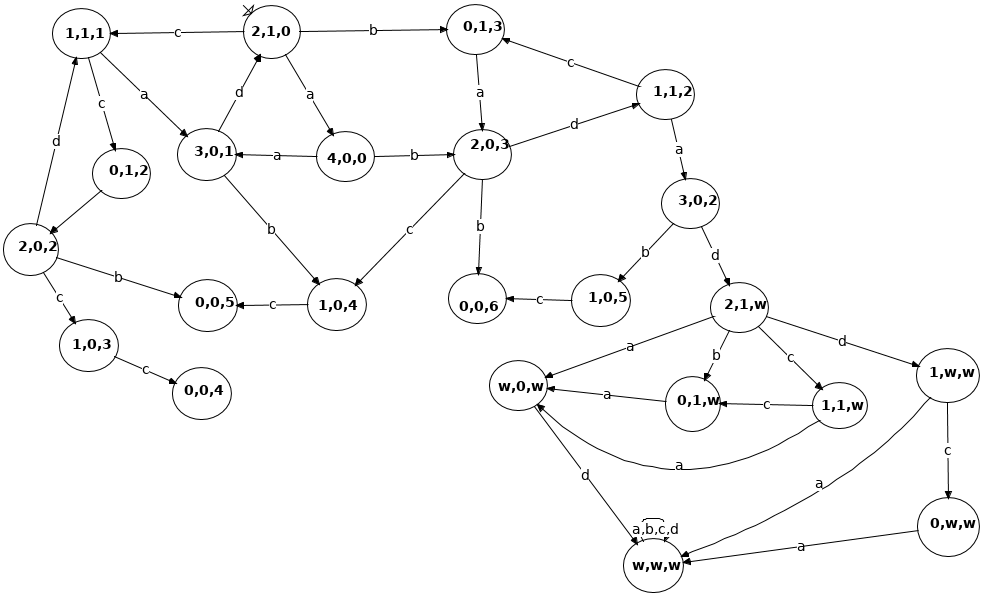
\includegraphics[scale=0.5]{netz.png}
\end{document}